%% Copernicus Publications Manuscript Preparation Template for LaTeX Submissions
%% ---------------------------------
%% This template should be used for copernicus.cls
%% The class file and some style files are bundled in the Copernicus Latex Package which can be downloaded from the different journal webpages.
%% For further assistance please contact the Copernicus Publications at: publications@copernicus.org
%% http://publications.copernicus.org


%% Please use the following documentclass and Journal Abbreviations for Discussion Papers and Final Revised Papers.


%% 2-Column Papers and Discussion Papers
\documentclass[gmd, manuscript]{copernicus}



%% Journal Abbreviations (Please use the same)

% Atmospheric Chemistry and Physics (acp)
% Advances in Geosciences (adgeo)
% Advances in Statistical Climatology, Meteorology and Oceanography (ascmo)
% Annales Geophysicae (angeo)
% ASTRA Proceedings (ap)
% Atmospheric Measurement Techniques (amt)
% Advances in Radio Science (ars)
% Advances in Science and Research (asr)
% Biogeosciences (bg)
% Climate of the Past (cp)
% Drinking Water Engineering and Science (dwes)
% Earth System Dynamics (esd)
% Earth Surface Dynamics (esurf)
% Earth System Science Data (essd)
% Fossil Record (fr)
% Geographica Helvetica (gh)
% Geoscientific Instrumentation, Methods and Data Systems (gi)
% Geoscientific Model Development (gmd)
% Geothermal Energy Science (gtes)
% Hydrology and Earth System Sciences (hess)
% History of Geo- and Space Sciences (hgss)
% Journal of Sensors and Sensor Systems (jsss)
% Mechanical Sciences (ms)
% Natural Hazards and Earth System Sciences (nhess)
% Nonlinear Processes in Geophysics (npg)
% Ocean Science (os)
% Primate Biology (pb)
% Scientific Drilling (sd)
% SOIL (soil)
% Solid Earth (se)
% The Cryosphere (tc)
% Web Ecology (we)


\begin{document}

\linenumbers

\title{An automatic and effective parameter optimization method for model tuning}


% % \Author[affil]{given_name}{surname}

\Author[1]{Tao}{Zhang}
%\Author[2]{Feng}{Xie}
%\Author[2]{Lijuan}{Li}
%\Author[1]{Wei}{Xue}
% %\Author[]{}{}

\affil[1]{Tsinghua}
%\affil[2]{LASG}
% %\affil[]{ADDRESS}

% %% The [] brackets identify the author with the corresponding affiliation. 1, 2, 3, etc. should be inserted.



\runningtitle{TEXT}

\runningauthor{TEXT}

\correspondence{Tao Zhang (t-zhang11@mails.tsinghua.edu.cn)}



% \received{}
% \pubdiscuss{} %% only important for two-stage journals
% \revised{}
% \accepted{}
% \published{}

% %% These dates will be inserted by Copernicus Publications during the typesetting process.


% \firstpage{1}

\maketitle
 

\begin{abstract}  

Physical parameterizations in General Circulation Model (GCM), having various uncertain parameters, greatly impact model performance and model climate sensitivity.  Traditional manual and empirical tuning of these parameters is time consuming and ineffective. In this study, a ``three-steps'' methodology is proposed to automatically and effectively obtain the optimum  combination of some key parameters in cloud and convective parameterizations based on a comprehensive objective evaluation metrics. It is found that the optimum combination of these parameters determined using this method is able to improve the model overall performance by 9\% in a GCM. The method can be easily applied to other GCMs to speed up model development process, especially regarding unavoidable comprehensive parameters tuning in model development.

\end{abstract}


\introduction  %% \introduction[modified heading if necessary] 

Due to current model resolution, GCMs need to parameterize various sub-grid scale processes. However, due to the complexities involved in these processes, there are various empirical determined parameters, especially within cloud and convective parameterizations. Sub-grid scale physical processes are presented as empirical or statistic parameters in climate system models \citep{hack1994climate}. Physical parameterizations aims to approximate the overall statistical outcomes of various sub-grid scale physics \citep{williams2005modelling}. Consequently, these parameterizations introduce uncertainties  to climate simulations using climate system models \citep{warren1979seasonal}. In general, these new uncertain parameters are required to be calibrated or constrained when new parameterization schemes are integrated into models \citep{li2013evaluation}.


Traditionally, the uncertain parameters are manually tuned by comprehensive comparison of model simulations with available observations. Such an approach is subjective, labor intensive, and hard to be extended \citep{hakkarainen2012closure, allen2000quantifying}. Currently, the automatic parameter calibration technique is a hot topic in uncertainty quantification of climate system model. The previous work focuses on the method of posterior range and probability, optimization algorithms, and data assimilation technique. The first class method, the optimization parameters confidence range is evaluated based on likelihood and Bayesian estimation. \cite{cameron1999flood} improves the forecast by the generalized likelihood uncertainty estimation (GLUE) \citep{beven1992future}, a method of obtaining parameters uncertain range of a specified confidence level. The Bayesian Markov chain Monte Carlo (MCMC) \citep{gilks2005markov} is widely used to obtain posterior probability distribution from prior knowledge. \cite{sun2013inverse} demonstrates the possibility of calibration of hydrologic in the CLM4  parameters with an Metropolis-Hasting algorithm, based on the MCMC approach. \cite{hararuk2014evaluation} calibrates soil C data in CLM-CASA model, a global land model consisting of biogeophysics and biogeochemistry processes using an adaptive Metropolis (AM) algorithm \citep{gilks2005markov}. \cite{jackson2008error} obtains parameters posterior probability  from clouds and convection physical process in CAM3.1 by Multiple Very Fast Simulated Annealing (MVFSA) to optimize a comprehensive metrics, including  cloud, radiation, temperature, precipitation, wind, as  well as humidity variables. This method is one to two orders of magnitude faster than the Metropolis-Hasting algorithm \citep{jackson2004efficient}. However, these methods only determine the likely area, can not directly specify a combination of uncertain parameters with a minimum metrics value. Meanwhile, the posterior distribution heavily depends on  the assuming the likelihood function.

The second class method, the optimization algorithms search the maximum or minimum metrics value in the given parameters space. \cite{severijns2005optimizing} calibrates parameters of radiation,  clouds, and convection in Speedy with downhill simplex \citep{press1992numerical,nelder1965simplex}, to improve the radiation budget at the top of the atmosphere and at the surface, and the  large scale circulation. Downhill simplex is a fast convergence algorithm when the parameters space is not high. But it is a local optimal algorithm, and difficult to search the global optimal solution.\cite{yang2013uncertainty} uses the  simulated stochastic approximation annealing (SSRR) \citep{liang2013simulated}  to tune the parameters of Zhang-McFarlane convection scheme to improve convection on the global circulation and climate. \cite{yang2014calibration}  uses the MVFSA algorithm to calibrate a convective parameterization scheme in the WRF model. However, the SSRR requires at least ten thousands steps to get a stable solution \citep{liang2013simulated}, and the MVFSA also requires thousands steps \citep{jackson2004efficient}. 	\cite{gill2006multiobjective} calibrates the SACSMA and SVM by multi-objective particle swarm optimization (MOPSO) . This algorithm requires dozens of individual cases in the each iteration, leading to high computational cost, compared with the downhill simplex, SSRR, and MVFSA, which need only one case. 

Another class method, data assimilation method becomes another research direction of parameters calibration. \cite{aksoy2006ensemble} estimates the parameter uncertainty of MM5 by the Ensemble Kalman Filter (ENKF). \cite{santiti2013simulated} presents a two-stage filtering for the joint state-parameter estimation with a combination method of the particle filtering (PF) and ENKF.  The same as the MOPSO method, ENKF and PF require  dozens of individual cases in each iteration. 
%the fifth-generation nonhydrostatic mesoscale model

The Atmospheric General Circulation Models (AGCM) is a strong nonlinear relationship system. Likewise, taken into account high dimensions of uncertain parameters space, the mentioned methods require long iterations for convergence. More seriously, the AGCMs require at least five years simulations to get the significant results(spin up?), spending around several hours. Therefore, the above work  is  time consuming and ineffective to calibrate the uncertain parameters. 


We propose a ``three-steps'' strategy. In the first step, a global sensitivity analysis method, Morris \citep{morris1991factorial,campolongo2007effective}, eliminates the insensitivity parameters by analyzing  the main and interaction effects among parameters. Another global method, Sobol \citep{sobol2001global}, is used to justify the Morris method. The downhill simplex algorithm is used to tune, because of its computational effect for dimension reduced parameters. Due to the initial values sensitivity to performance, a step of pre-processing initial values of the downhill simplex is conducted. Taken into account the complex configuration and manipulation of the ``three-steps'', invoking parameters sampling, namelist reset, models running simultaneously, optimization iteration, sensitivity analysis, as well as metrics diagnostics, a automatic workflow is provided to make the calibration process more efficient. The ``three-step'' calibration strategy is applied to GAMIL2, a Grid-point Atmospheric Model developed by State Key Laboratory of Numerical Modeling for Atmospheric Sciences and Geophysical Fluid Dynamics, Institute of Atmospheric Physics, China, to improve the comprehensive simulation performance of the climate mean state.

Section 2 describes the details of the method and the structure of the automatic workflow. The application of the method in a GCM is presented in section 3 with a summary and discussion in section 4.

\section{Method}
The ``three-steps'' provides an effective and efficient calibration strategy. It aims at reducing the dimension of tuning space by eliminating the insensitivity parameters, and reducing the iteration steps by pre-processing initial values of optimal algorithms. An inexpensively computational algorithm, downhill simplex, is used to search the optimal solution.

\subsection{Sensitive parameter determination}
The number of uncertain parameters in physical parameterizations of the climate system model is large. Most optimization algorithms, such as particle swarm optimization (PSO), downhill simplex, and simulated annealing mentioned above are ineffective in the high dimension space. The higher dimension space, the more iterations are needed.  Additionally, some components of climate system model, such as atmosphere and ocean, require a long time to get the significant simulations (spin up?). Therefore, it suffers to an extremely calibration computational cost.  It is necessary to reduce the parameters dimension. 

The Morris method \citep{morris1991factorial,campolongo2007effective}, is a qualitative global sensitivity method. The advantage of this method is that not only the single parameter sensitivity can be presented, but also the interactive sensitivity among parameters can be described. 

The sampling strategy is based on Morris’s one-step-at-a-time (MOAT) experiment design using relatively few samples. It only needs  $(n+1) \times M$ points, where n is the number of calibration parameters and M is number of trajectories, usually 10-20. Consider the n parameters $x_i (i=1,...,n)$, normalized to [0,1]. The influence of each variables is defined as a elementary effect, show as equation (1), where $\Delta$ is the value of $1/p-1, ..., p-2/p-1$, and p is the sampling level. The starting point of a trajectory is selected randomly and completed it by adjusting one unchanged parameter value at a time in a random order, consisting $n+1$ samplings. The mean of $|d_j|$ stands for the main effect of a single parameter, and the standard deviation presents the interactive effect of multiple parameters. Therefore, those with low mean and low standard deviation will be eliminated. In this paper, parameters in table 2 are required to analysis sensitivity. We sample 80 points, and the results are showed in Figure 1. The insensitivity parameters, ke, capelmt and c0 of shallow convection, are removed.

\begin{align}
& d_{ij} = \frac{y(X_1,...,X_j+\Delta,...,X_N)-y(X_1,...,X_j,...,X_N)}{\Delta} \\
& \mu_j = avg(|d_{i,j}|), \sigma_j = stddev(d_{i,j}) 
\end{align}

To justify the Morris method, we compare the results a benchmark method, Sobol \citep{sobol2001global}. It is a quantitative method based on variance decomposition requiring more samples than the Morris, with a higher computation cost. The variance of model output can be decomposed as equation (3), where n is the number of parameters, and $V_i$ is the variance of the $i_{th}$ parameter, and $V_{ij}$ is variance of iterative effect between the $i_{th}$ and $j_{th}$ parameters, and so on. The total sensitivity effect can be presented as equation (4), where $V_{-i}$ is the total variance except for the $x_i$ parameter. The Sobol results are showed as figure 2.  The screened out parameters are the same as the Morris.

\begin{align}
& V = \sum_{i=1}^n V_i + \sum_{1 \leq i < j \leq n} V_{ij} + ... + V_{1,2,...,n}  \\
& S_{T_i} = 1 - \frac{V_{-i}}{V} 
\end{align}
$V_{-i}$ is the total variance except for $X_i$

\subsection{A novel downhill simplex optimization method with the most appropriate initial value}

Parameter tuning in climate system model is a global scale optimization problem in theory.  But the common evolutionary algorithms, such as genetic algorithm \citep{goldberg1989messy}, differential evolutionary (DE) \citep{storn1995differential} , and PSO, generally requires at least  thousands of iterations to get a stable global solution and a population of individuals in each iterations, causing large computation cost \citep{hegerty2009comparative,shi1999empirical}. It is infeasible to get the best optimization simulation by calibrating parameters. Therefore, to acquire a more optimal result in limited iterations is more practical.

In this paper, we use and improve the downhill simplex to tune the uncertain parameters .The downhill simplex searches the optimal solution by changing the shape of a simplex, which represents the optimal direction and step length. A simplex is a geometry, consisting of $N+1$ vertexes and their interconnecting edges, where N is the number of calibration parameters screened by the 2.1 section. The vertexes stand for the pair of a set of parameters and its metrics. The new vertex is determined by expanding and shrinking the vertex with the highest metrics value, restructuring the new simplex. The details of the downhill simplex are described in \cite{press1992numerical} and \cite{nelder1965simplex}


The convergence performance of the downhill simplex is sensitivity with its initial values. The parameter combinations with the smaller metrics will be selected.  Because if the initial simplex has a large span, it can jump out the local searching area by reflecting geometry and retractable transformation. In this case, the downhill simplex has a good global optimization capability at a low starting point. Otherwise, it oozes down the valley area and traps into the local optimal space. Therefore, the selected initial values can fast search the local optimal simulations.  The initial values are determined by the full factor sampling method within the full range of the sensitivity parameters.  The full factor method is an equilibrium distance sampling strategy, and is suitable to analysis the parameters values sensitivity in a low dimension space. We use it to sample in the given range as shown table 1, and refine sampled in a sensitivity range.


Besides, the inappropriate initial values may lead to the ill-conditioned simplex geometry. It means that some parameters keep the same value in the initial values. These parameters cannot change in the optimal algorithm. Consequently, as much as different sampled parameters values are required to select to improve the parameters freedom of initial values. This procedure is presented as the initial values pre-processing of downhill simplex algorithm.


\subsection{Implementation of the end-to-end automatic calibration workflow}

Though the ``three-steps'' strategy is an effective calibration discussed in section 4.1, it invokes in many messy manipulations, including parameters sampling, parameter values configuration of models, multi models running simultaneously, metrics diagnostic, parameters sensitivity analysis, selecting the initial values of tuning algorithms, and the optimal results analysis. These operations no doubt lead to the inefficient calibration manipulation without an automatic workflow.

The common uncertainty quantification toolboxes, such as Problem Solving environment for Uncertainty Analysis and Design Exploration (PSUADE) \citep{tong2005psuade}, Design Analysis Kit for Optimization and Terascale Applications (DAKOTA) \citep{eldred2007investigation}, support various uncertainty analysis methods, like parameter sampling, sensitivity analysis, numerical optimization, and response surface analysis.  These tools provide the function interfaces and an automatic workflow including parameter sampling, application running, and results collecting and analyzing. However, they cannot support multiple cases running simultaneously, the duplicate samples reducing, flexible optimization algorithm, and the climate mechanism analysis. Therefore, these tools are inefficient and inflexible to calibrate the uncertain parameters in climate system model.   

Based on the manipulation of parameters calibration in climate system model and the operations of the ``three-steps'', we design and implement the end-to-end automatic workflow. Users only require to specify the calibration parameters of interest and their initial value range. The workflow can automatically execute the ``three-steps'' calibration strategy, and produce the optimal parameters and its corresponding diagnostic results. Besides, this workflow is opening system that the above common tools, PSUADE, DAKOTA, and others toolboxes, can be integrated.

The structure of the automatic workflow is presented as in figure 1. It consists of four components, dimension reduction, calibration algorithms, post-processing, and tasks schedule. The dimension reduction module provides Morris and Sobol sensitivity analysis methods, and various sampling method, such as full factor, Latin Hypercube (LH), Morris one-at-a-time (MOAT) , and Central Composite Designs (CCD). Meanwhile, this module supports eliminate duplicate sampling points, reducing the unnecessary computing loads. As well, MCMC method based on adaptive Metropolis-Hastings algorithms is also provided to get the posterior distribution of uncertain parameters. The calibration algorithm module offers the local and global optimization algorithms. To take full use of computation resource, the scheduler module schedule as many as application cases running simultaneously. The post-processing module is response for metrics diagnostic, reanalysis and observation data management. Additional, all the intermediate metrics and their corresponding parameters are stored in DATABASE, used for posterior knowledge analysis.


\section{Application in GAMIL2 model} 
\subsection{Model description} 
In this paper, the Grid-point Atmospheric Model of IAP LASG version 2 (GAMIL2) is used. It takes
part in the Atmospheric Model Inter-comparison Project (AMIP) of IPCC AR5, Cloud Feedback Model
Inter-comparison Project (CFMIP) and  Coupled Model Intercomparison Project Phase 5 (CMIP5) as an
atmospheric component of Flexible Global-Ocean-Atmosphere-Land System Model grid version 2
(FGOALS-g2). The horizontal resolution is 2.8 x 2.8, with 26 vertical levels. The dynamical core of
GAMIL2 is a finite difference scheme, and conserves mass and effective energy
\citep{wang2004design}. The moisture equation adopts the two- step shape-preserving advection
scheme \citep{rucong1994two}. Compared with GAMIL1, the previous version, GAMIL2 has modifications on cloud-
related process \citep{li2013evaluation}, such as the deep convection parameterization
\citep{zhang2005effects}, the convective cloud fraction \citep{xu1991evaluation}, and the cloud
microphysics \citep{morrison2008new}. The initial calibrated parameters are selected  from deep
convection, shallow convection, cloud fraction, cloud microphysical processes and boundary layer
scheme, as table 1 shown. The default parameter values are the configuration of the standard
version, which takes part in IPCC AR5 and is called CNTL.


\subsection{Evaluation data and metrics}

Wind, humidity, and geopotential height derive from the European Center for Medium-Range
Weather Forecasts (ECMWF) Re-Analysis (ERA) - Interim reanalysis, 1989 to 2004 and 1.5x1.5
horizontal resolution \citep{simmons2007era}. The precipitation comes from the Global Precipitation
Climatology Project (GPCP), 1989 to 2004 and 2.5x2.5 horizontal resolution \citep{adler2003version}
. The radiation variables use the Earth Radiation Budget Experiment (ERBE), 1985 to 1989  and
1.875x1.875 horizontal resolution \citep{barkstrom1984earth}. The climate mean state of
observational data are require to  remap to the grid of GAMIL2. However, the duration of simulation
(2000-2004)  is inconsistent with the observational data. We conduct a long simulation (1989-2004)
with the optimal parameters to insure the tuning parameters validity. The results show the
consistent with the short simulation.

A comprehensive metrics, including wind, temperature, humidity, geopotential height, precipitation
and radiation flux is used to quantitatively evaluate the simulation performance, to improve
overall simulation skills \citep{murphy2004quantification,gleckler2008performance,reichler2008well}
. These variables are shown as table 2. The model starts up in the 2000th year, and simulates 5
years. Climate mean state of the last three years is used to diagnostic metrics. The
calibration RMSE is defined as the spatial standard deviation (SD) of model simulation against
observations, as equation (5) \citep{taylor2001summarizing,yang2013uncertainty}. In the propose  of
integrating the 16 variables into a unique metrics, the SD of default GAMIL2  simulations against
observations is used to scale each variable calibration RMSE, as equation (6). Finally, the 
metrics is computed as the average value of each scaling variable factor, as equation (7). 
Therefore, if the metrics is lower than one, the model performance have been improved.

\begin{align}
(\sigma_m^F)^2 &= \sum_{i=1}^l w(i)(x_m^F(i) - x_o^F(i))^2 \\
(\sigma_r^F)^2 &= \sum_{i=1}^l w(i)(x_r^F(i) - x_o^F(i))^2 \\
\chi^2 &= \frac{1}{N^F}\sum_{F=1}^{N^F} (\frac{\sigma_m^F}{\sigma_r^F})^2
\end{align}

$x_m^F(i)$ is the model outputs according to selected shown in the Table 2. $x_o^F(i)$ is the 
corresponding observation or reanalysis data. $x_r^F(i)$ is the reference results from CMIP5. w is 
the weight due to the different grid area. I is the total grid number in model. $N^F$ is the 
number of the chosen variables.


\section{The optimization results and mechanism analysis}

\subsection{Comparison the effective and efficient with different strategies}

We compare the effective and efficient performance among the ``three-steps'', ``two-steps'' of initial values pre-processing and down-hill simplex (Tao Zhang et al., Quantification and optimization of parameter uncertainty in the Grid-point Atmospheric Model GAMIL2, manuscript in review, 2014), and ``one-step'' directly using optimal algorithms with downhill simplex, DE and PSO. The ``two-steps'' and ``three-steps'' require extra twenty-five samples for the initial values pre-processing. Eighty samples for parameters space reducing are required for the ``three-steps''. The 3rd column in table 3 is the number of iterations before each method gets the optimal solution in the 2nd column. The real iteration steps are greater than the number in table 3. The size of population of DE and PSO is set as twelve. The effective of each strategy is evaluated by the optimal solution, and the efficiency is evaluated by the core hours, computed as $N_{step} \times N_{size} \times 30 \times 6$, where $N_{step}$ is the number of iterations, and $N_{size}$ is the size of population. The model runs as thirty processes, each assigned one core, and simulates five model years, about six hours. In the ``one-steps'' strategy, though the PSO gets a good optimal solution, it spends a expensive computational cost. On the contrary, the ``three-steps'' gets the best solution using half core hours than the PSO. The ``two-steps'' has the best efficiency, while the key factor, optimal solution is worse than the ``three-steps''.


\subsection{The optimal mechanism analysis}

Figure 4 exhibits the taylor diagram of the 16 variables of three years climate mean state from 2002 to 2004.  No variable of EXP becomes seriously worse than CNTL. Instead,  Zonal wind at 850hPa (U850),  Zonal wind at 200hPa (U200), Meridional wind at 850hPa (V850), Meridional wind at 200hPa (V200), and Specific Humidity at 400hPa (Q400) have been obviously improved. Figure 5 shows the metrics of each variables with the global, tropic, and northern / southern middle and high latitudes (NMHL / SMHL). Most variables of global are improved compared with CNTL. Specific Humidity at 400hPa (Q400) is the best improved. Two variables, Meridional wind at 200hPa (V200) and clearsky short wave net flux at TOA (FSNTOAC), keep the same magnitude. 850hPa and 200hPa temperature are worse than CNTL. From the spatial distribution perspective, the SMHL contributes the best improved


Figure 5 presents the improvement of the entire radiation variables. It could be attributed to the specific humidity and cloud improvement in the middle and upper troposphere. The EXP consumes the more water vapor and gets the better simulation than CNTL above 700hPa, shown as figure 6. The decrease of the atmospheric water vapor reduces the its greenhouse effect. Therefore, it emits the more outgoing long-wave radiation in clear sky, reducing the negative bias of clear sky long wave upward flux at TOA (FLUTC), shown as figure 8(a).


Compared with CNTL, the middle and high cloud significantly increase, as a result of the reducing rhminh parameter, shown as figure 7. Consequently, it enhances the blocking effect on the long wave upward flux at TOA (FLUT), reducing the FLUT in 30$^\circ$-60$^\circ$ of the southern and northern hemisphere, shown as figure 8(b). Taken into account the long wave cloud forcing (LWCF) computed as $FLUTC - FLUT$, the improvement of FLUTC in tropical is make up for the increasing bias of FLUT. Therefore, the LWCF in tropical stays the same with CNTL. But the LWCF in the middle and high latitudes is improved due to the improvement of FLUT in this area, shown as figure 8(c). 



\conclusions  %% \conclusions[modified heading if necessary]  

In this paper, we presents the ``three-steps'' strategy of uncertain physical parameters in
GAMIL2.The initial high parameters space is reduced by the global sensitivity methods, Morris and
Sobol. To improve the convergence speed of down-hill simplex, a initial values pre-processing
optimal algorithms is used based on the full factor sampling to evaluate the likely area of the
optimal solution. The experiment results show the ``three-steps'' outperforms the PSO and DE in
both of effective and efficiency. Though the ``two-steps'' has an advantage in efficiency, the
optimal solution is worse than the ``three- steps''. Besides, if the parameters dimension
increases, it may not get the best performance. Taken into account the complex configuration and
manipulation, we design and implement the automatic parameters calibration workflow to further
enhance operation efficiency and to support multi uncertainty quantification analysis and
calibration strategy. The optimal results of the ``three- steps'' demonstrate most of the variables
are improved compared with the CNTL, especially for the radiation variables, which present the
entirely improved. The mechanism analysis explores that the reduced simulation errors of water 
vapor has direct effect on the FLUT, and via cloud fraction indirectly influences the FLUTC. The 
LWCF is improved under the improved FLUT and FLUTC.

For future work, we plan to test the DE and PSO in the ``three-steps''. We will also develop the computation cheap surrogate model, because the high computational cost is the one of the biggest challenge for calibrating the climate system model. Besides, the optimal results need more mechanism analysis to deeply understand the model uncertain source.  
% \appendix
% \section{}    %% Appendix A

% \subsection{}                               %% Appendix A1, A2, etc.




% \begin{acknowledgements}
% TEXT
% \end{acknowledgements}


% %% REFERENCES

% %% The reference list is compiled as follows:

% %\begin{thebibliography}{}

% %\bibitem[AUTHOR(YEAR)]{LABEL}
% %REFERENCE 1
% %
% %\bibitem[AUTHOR(YEAR)]{LABEL}
% %REFERENCE 2
% %
% %\end{thebibliography}

% %% Since the Copernicus LaTeX package includes the BibTeX style file copernicus.bst,
% %% authors experienced with BibTeX only have to include the following two lines:
% %%
\bibliographystyle{copernicus}
\bibliography{uq}
%%
%% URLs and DOIs can be entered in your BibTeX file as:
%%
%% URL = {http://www.xyz.org/~jones/idx_g.htm}
%% DOI = {10.5194/xyz}


%% LITERATURE CITATIONS
%%
%% command                        & example result
%% \citet{jones90}|               & Jones et al. (1990)
%% \citep{jones90}|               & (Jones et al., 1990)
%% \citep{jones90,jones93}|       & (Jones et al., 1990, 1993)
%% \citep[p.~32]{jones90}|        & (Jones et al., 1990, p.~32)
%% \citep[e.g.,][]{jones90}|      & (e.g., Jones et al., 1990)
%% \citep[e.g.,][p.~32]{jones90}| & (e.g., Jones et al., 1990, p.~32)
%% \citeauthor{jones90}|          & Jones et al.
%% \citeyear{jones90}|            & 1990

\clearpage
%% FIGURES

%% ONE-COLUMN FIGURES

%f
\begin{figure}[t]
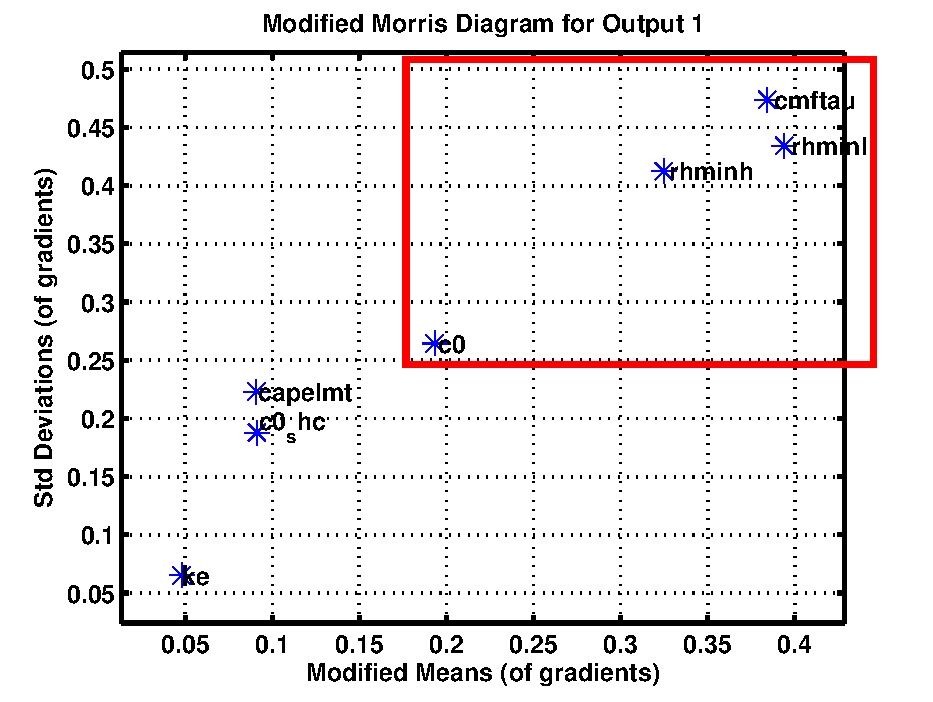
\includegraphics[width=8.3cm]{Morris}
\caption{Morris sensitivity scatter diagram. c0, rhminl, rhminh, and cmftau have the high sensitivity. ke, c0\_shc, and capelmt have the low sensitivity.}
\end{figure}

\begin{figure}[t]
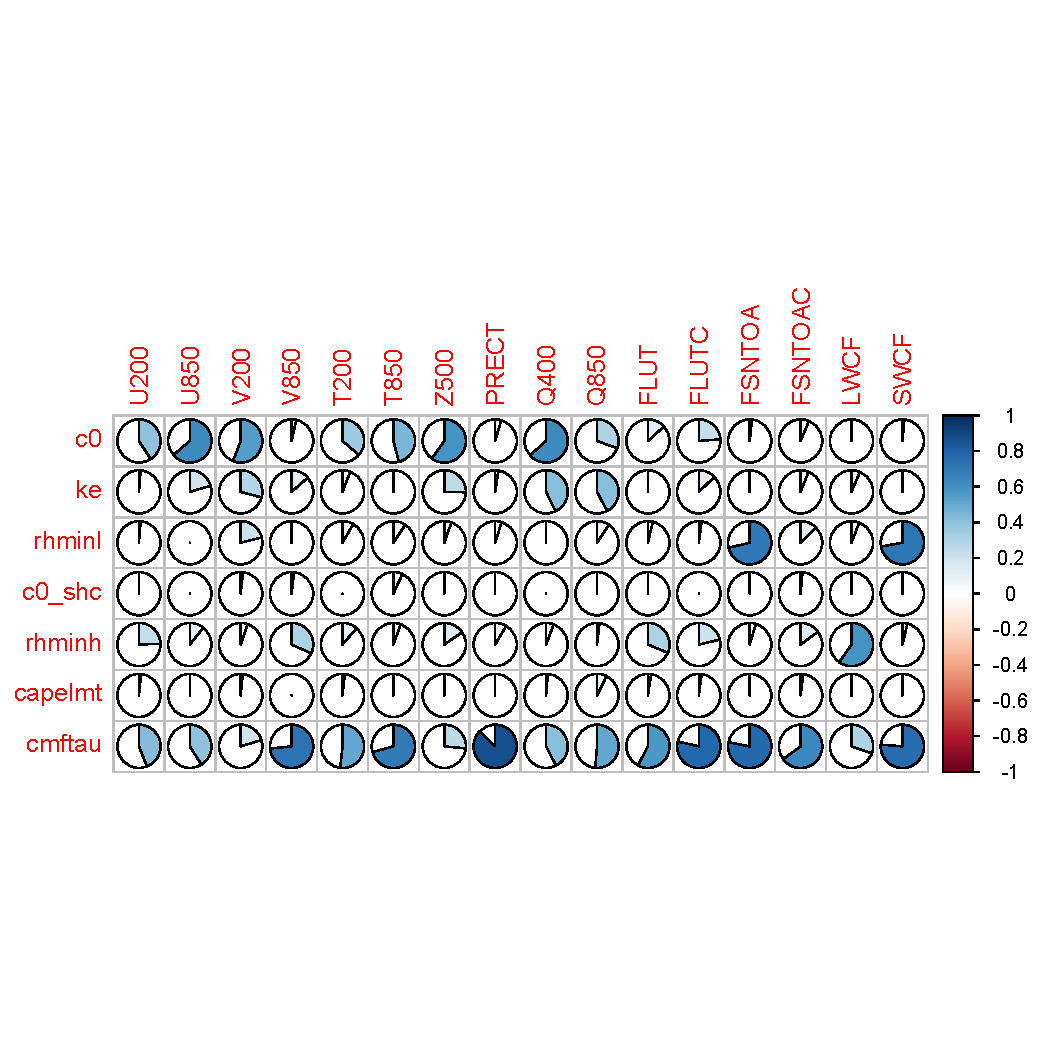
\includegraphics[width=8.3cm]{Sobol}
\caption{Sobol sensitivity results. The total sensitivity of ke, c0\_shc, and capelmt with regard to each variable is not more than 0.5.}
\end{figure}

\begin{figure}[t]
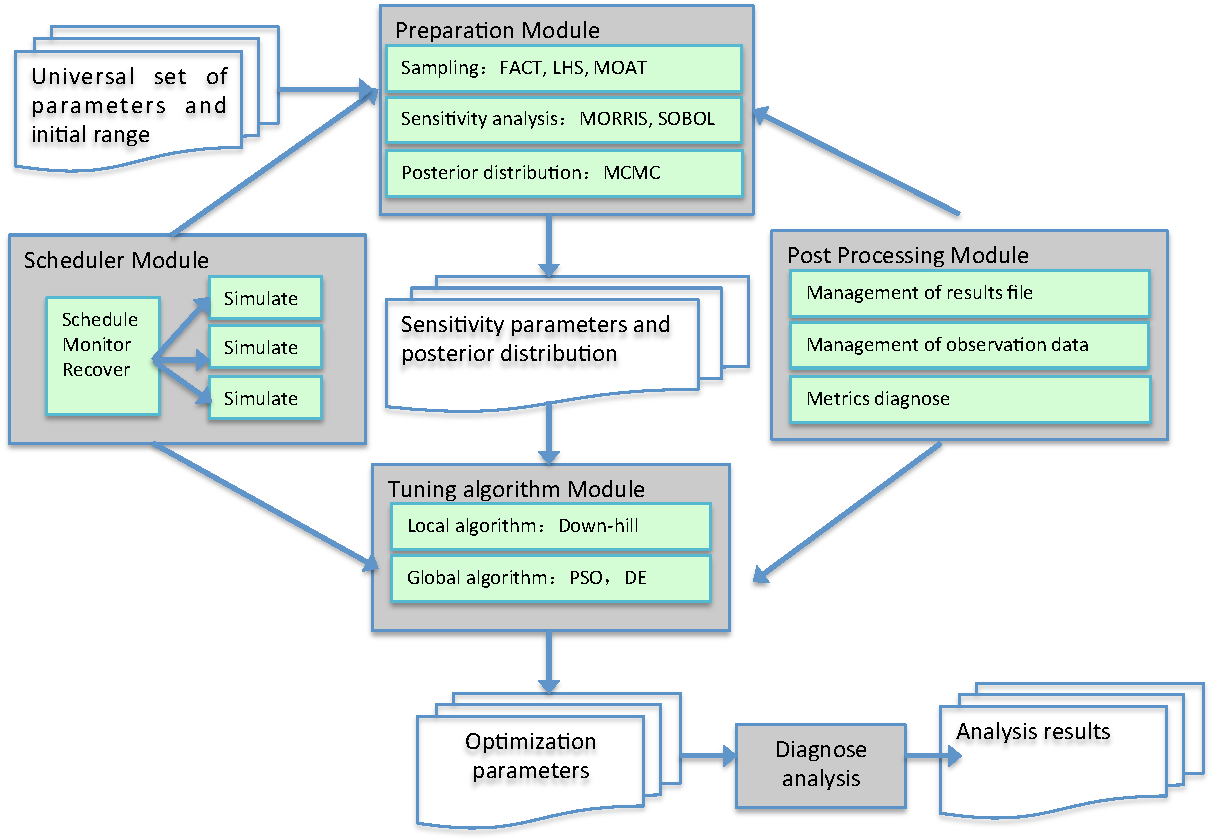
\includegraphics[width=15.3cm]{workflow}
\caption{The structure of the automatic calibration workflow}
\end{figure}

\begin{figure}[t]
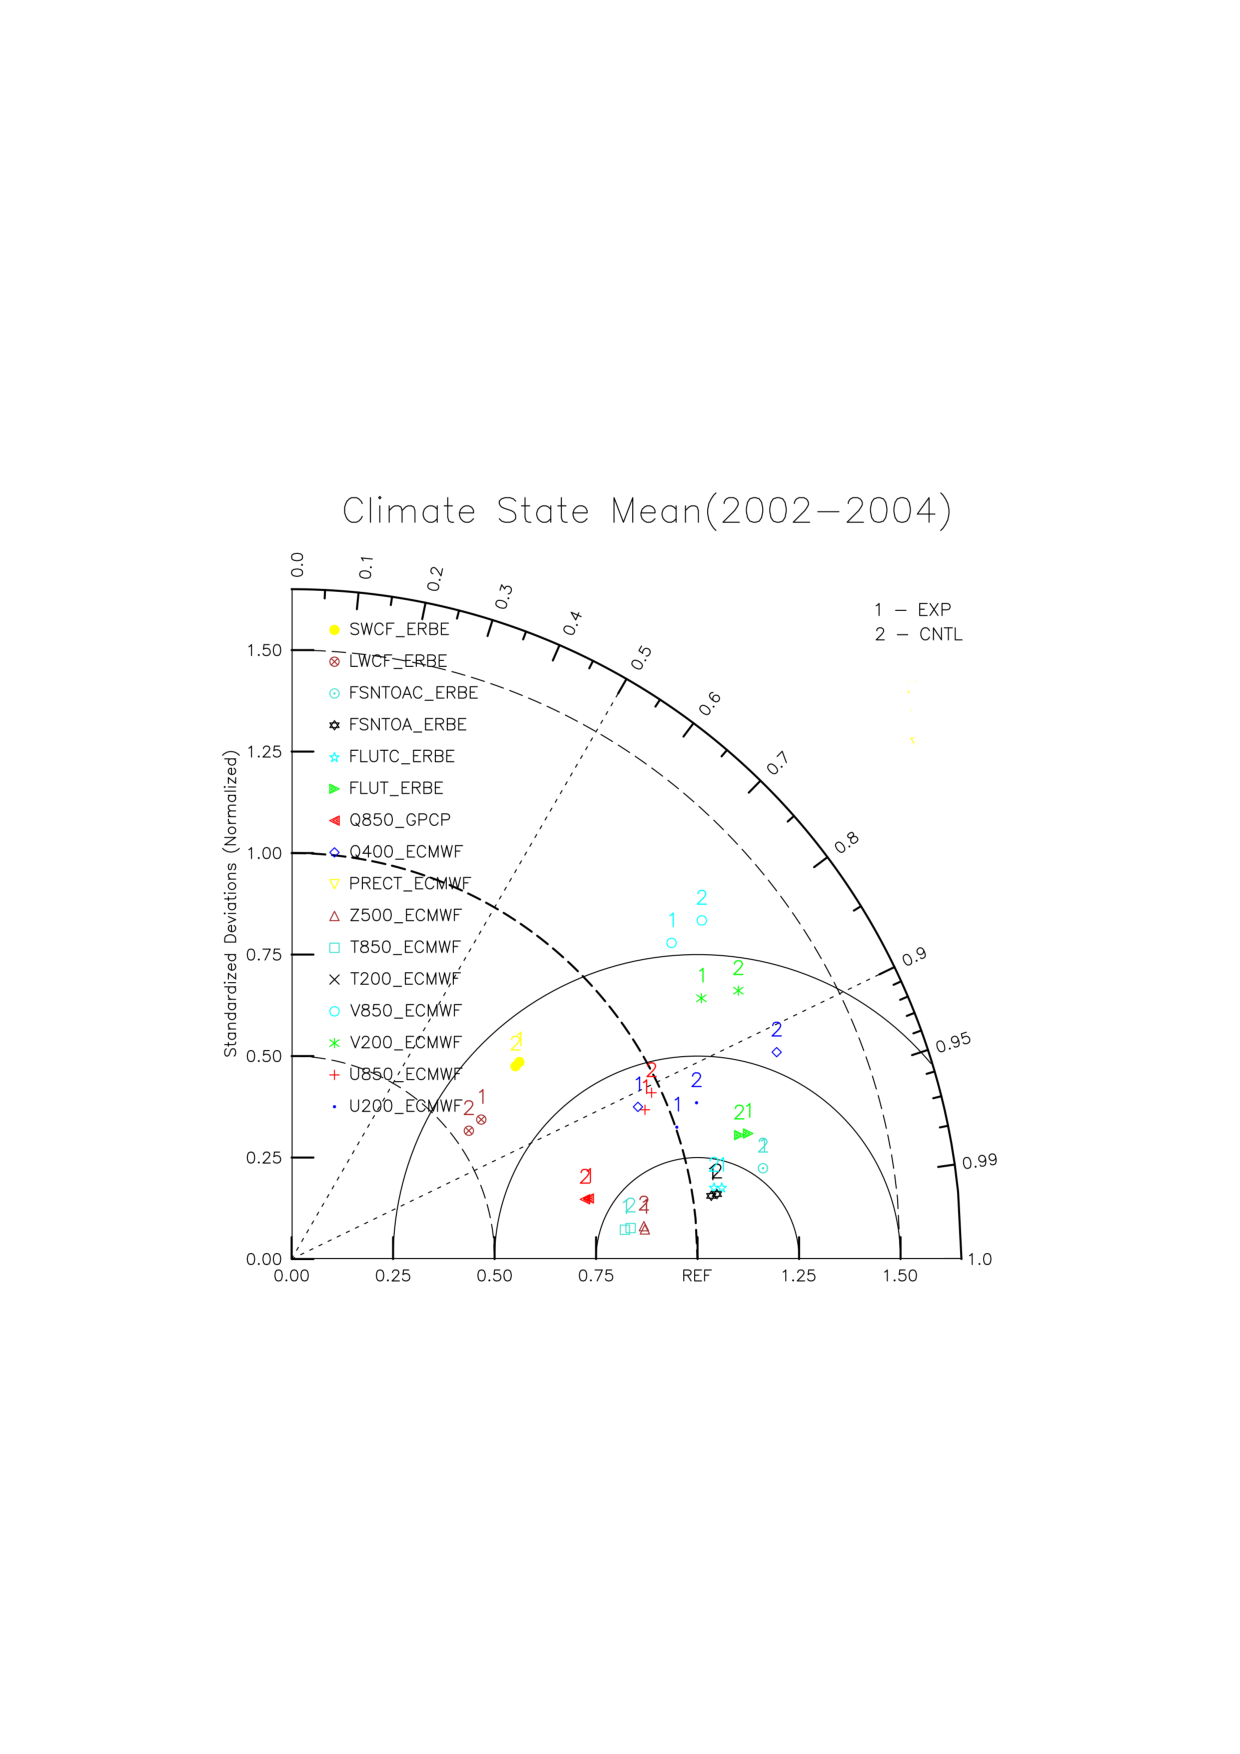
\includegraphics[width=12cm]{taylor}
\caption{Taylor diagram of each variables climate mean state from 2002 to 2004 of EXP and CNTL.}
\end{figure}

\begin{figure}[t]
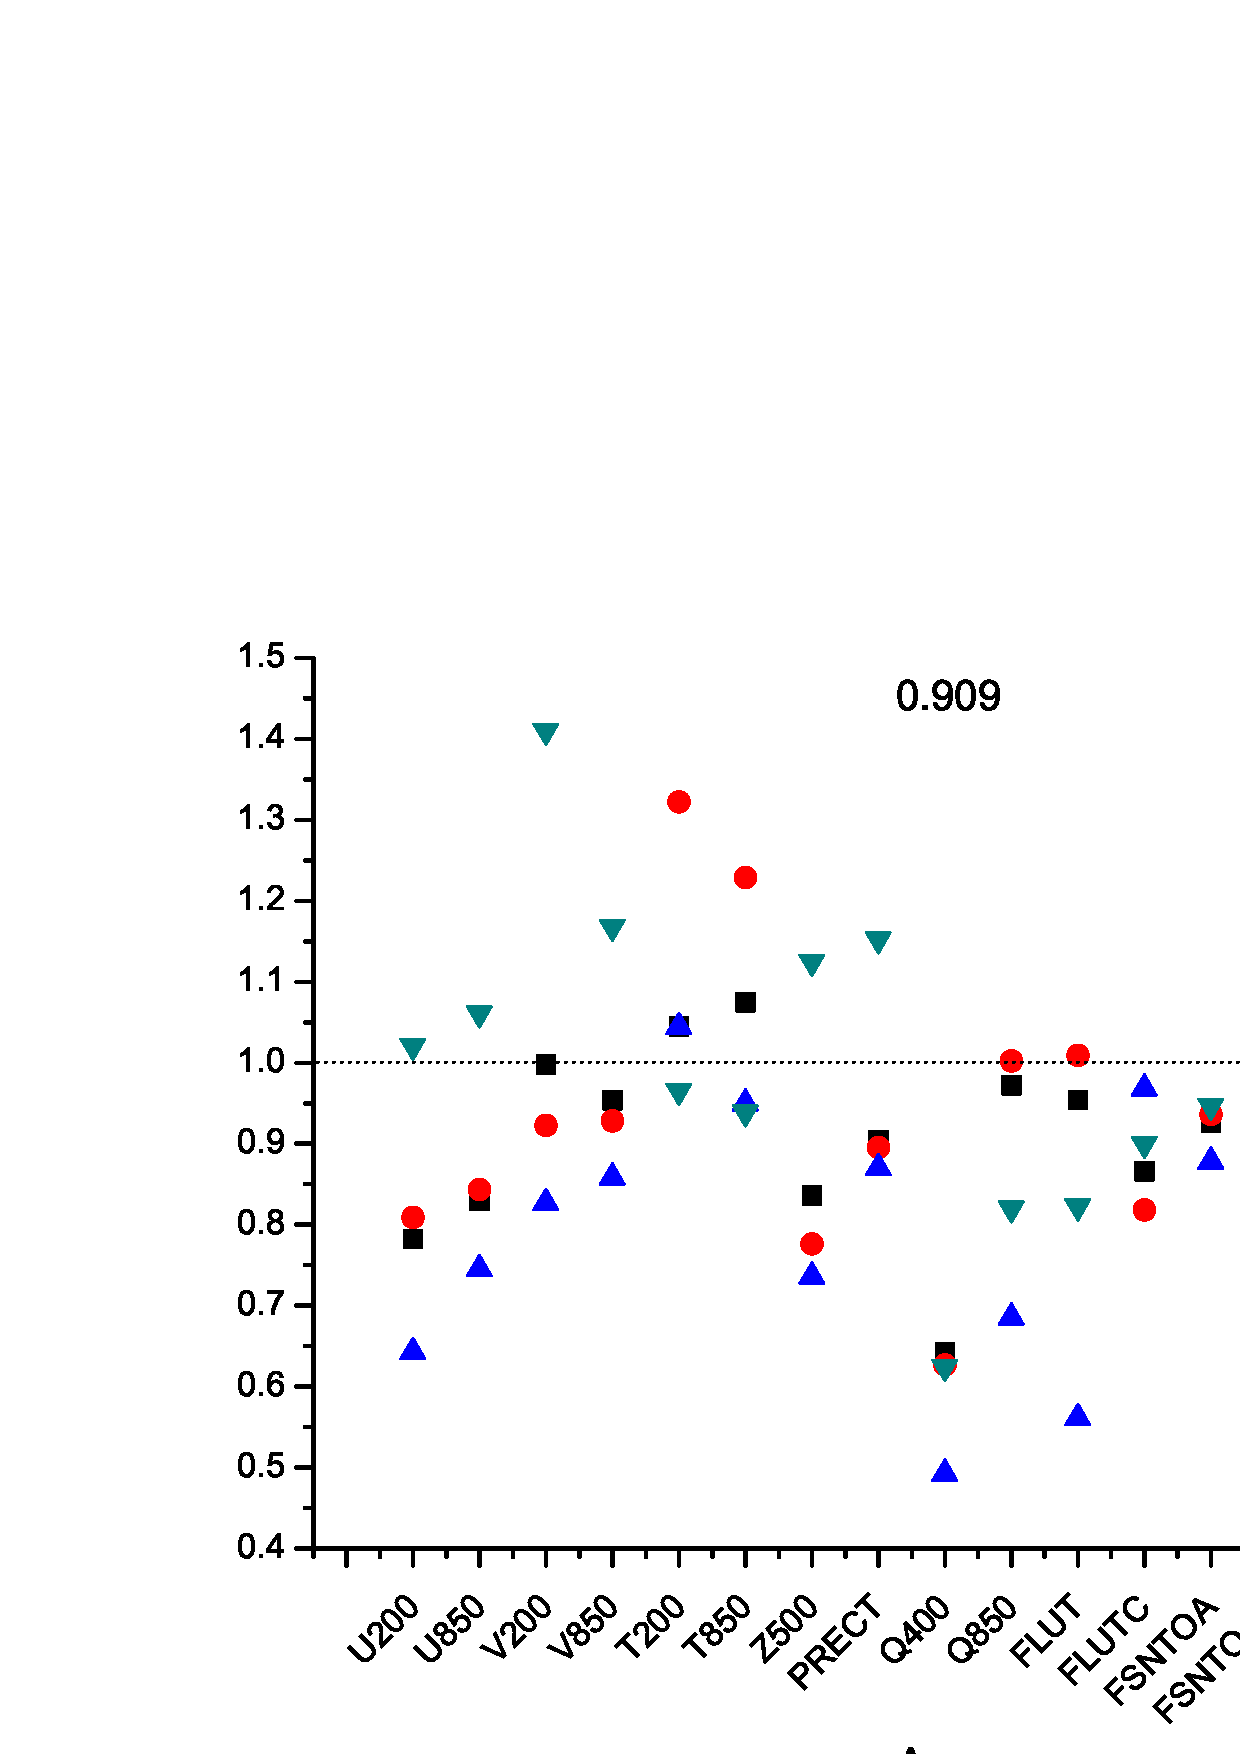
\includegraphics[width=15.3cm]{reg}
\caption{Metrics of each variables with the global, tropic, and northern / southern middle and high latitudes}
\end{figure}

\begin{figure}[t]
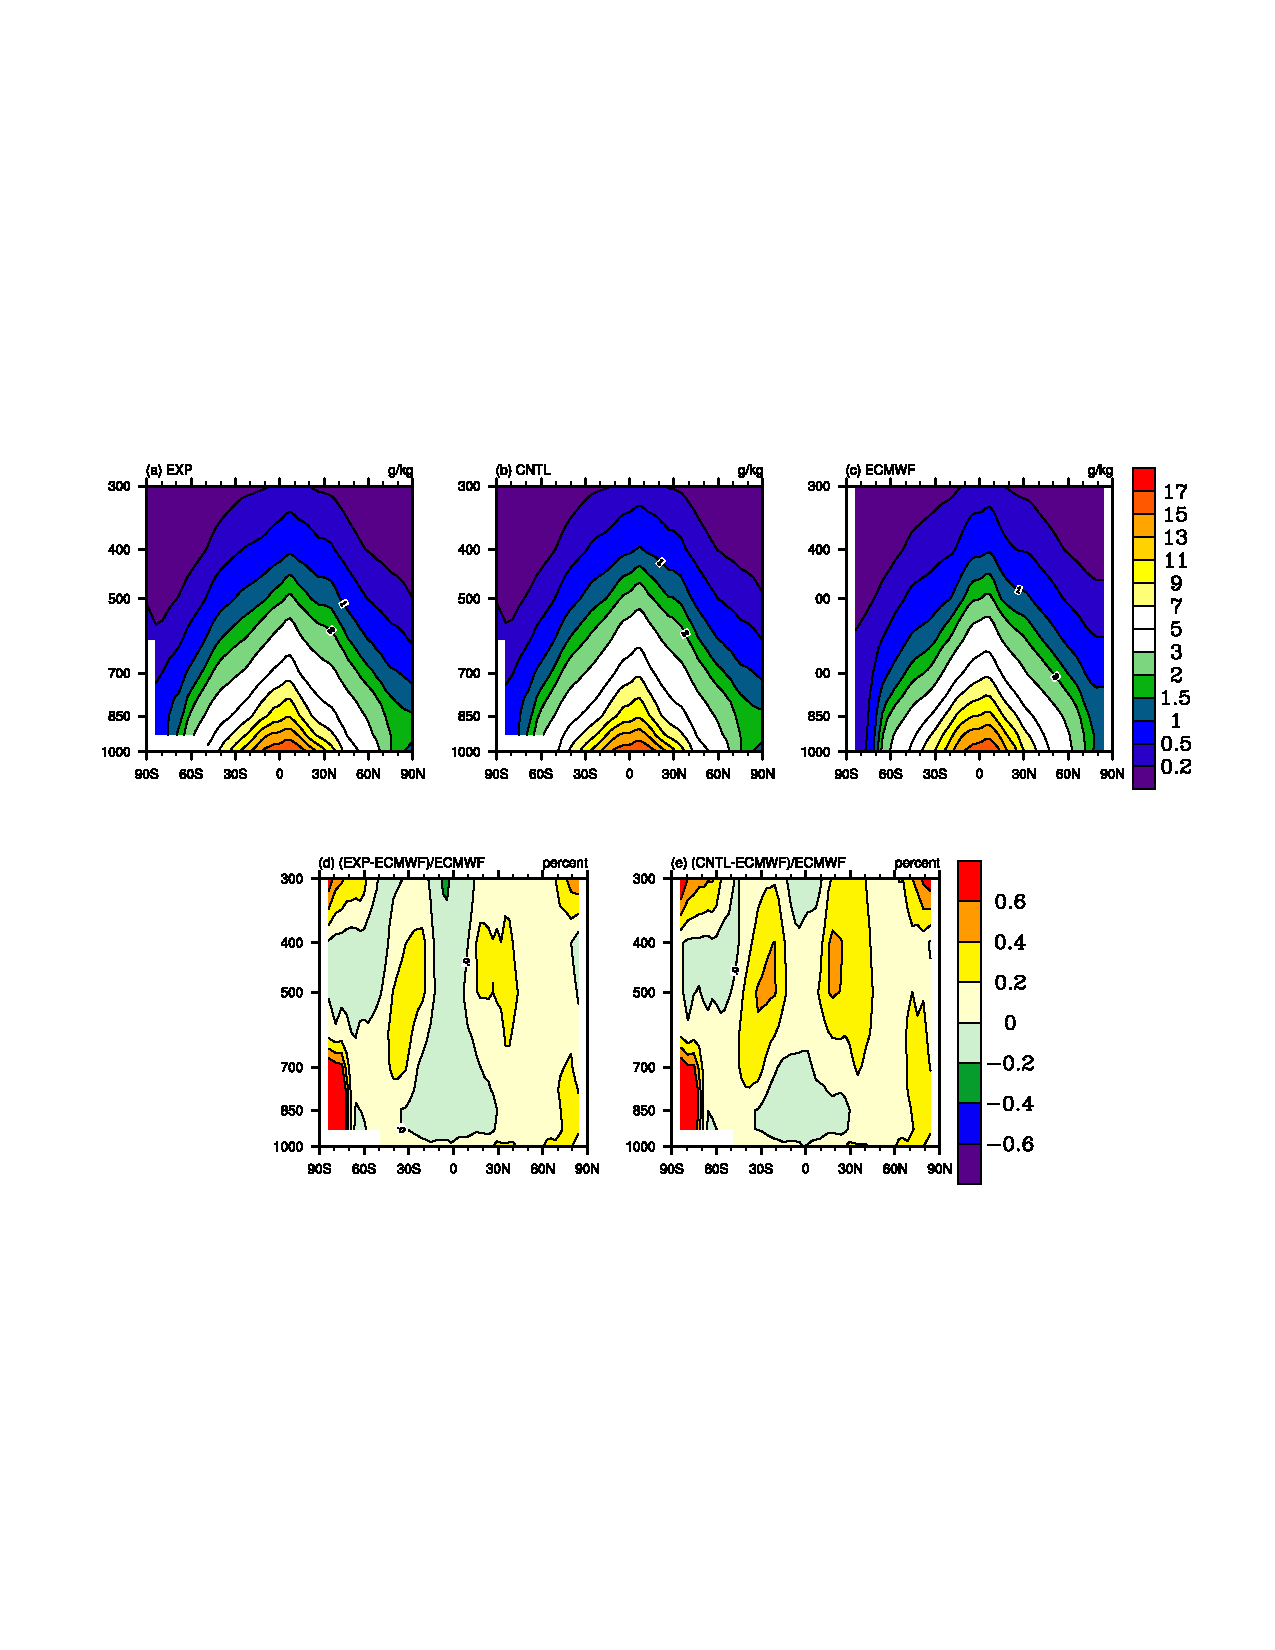
\includegraphics[width=15.3cm]{shum}
\caption{Pressure-latitude distributions of specific humidity of EXP (a), CNTL (b), observation (c), EXP-observation (d), and CNTL-observation (e).}
\end{figure}

\begin{figure}[t]
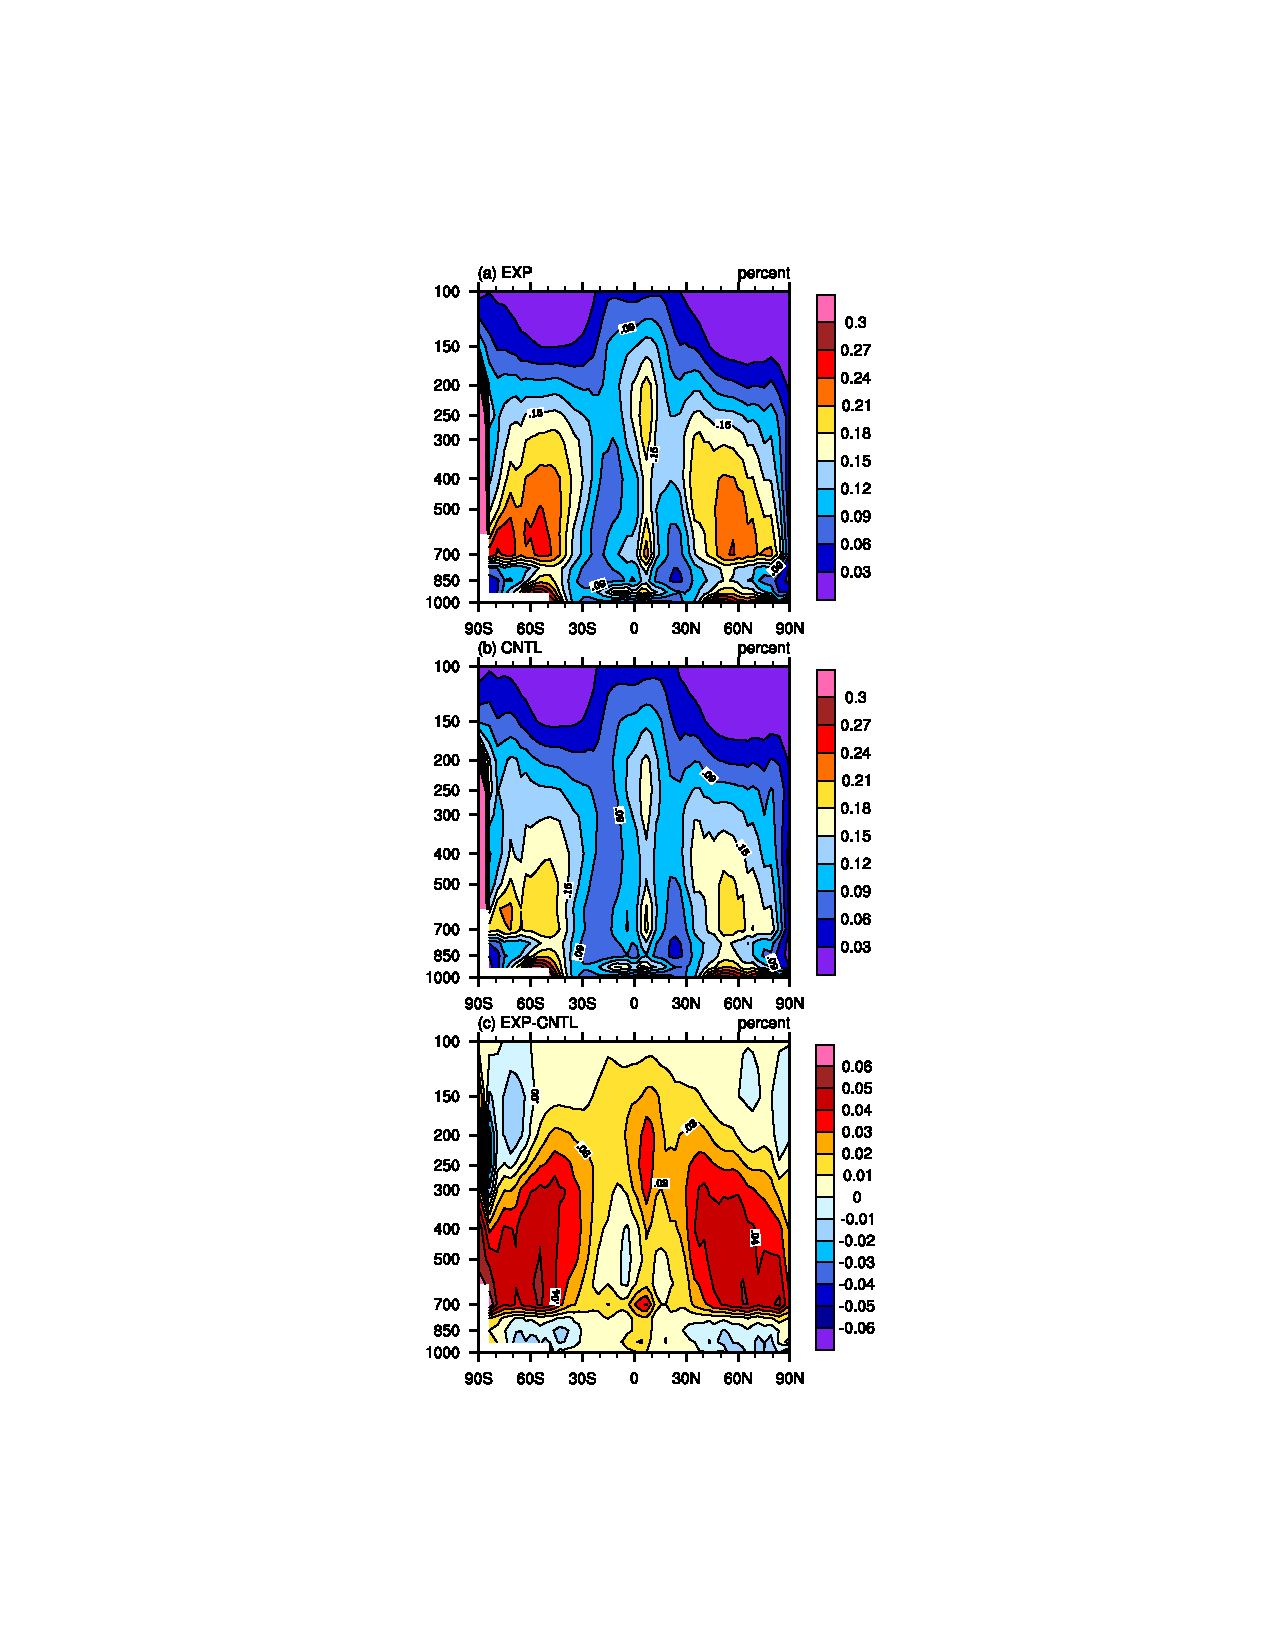
\includegraphics[width=15.3cm]{cloud}
\caption{Pressure-latitude distributions of cloud fraction of EXP (a), CNTL (b), and EXP-CNTL (c).}
\end{figure}

\begin{figure}[t]
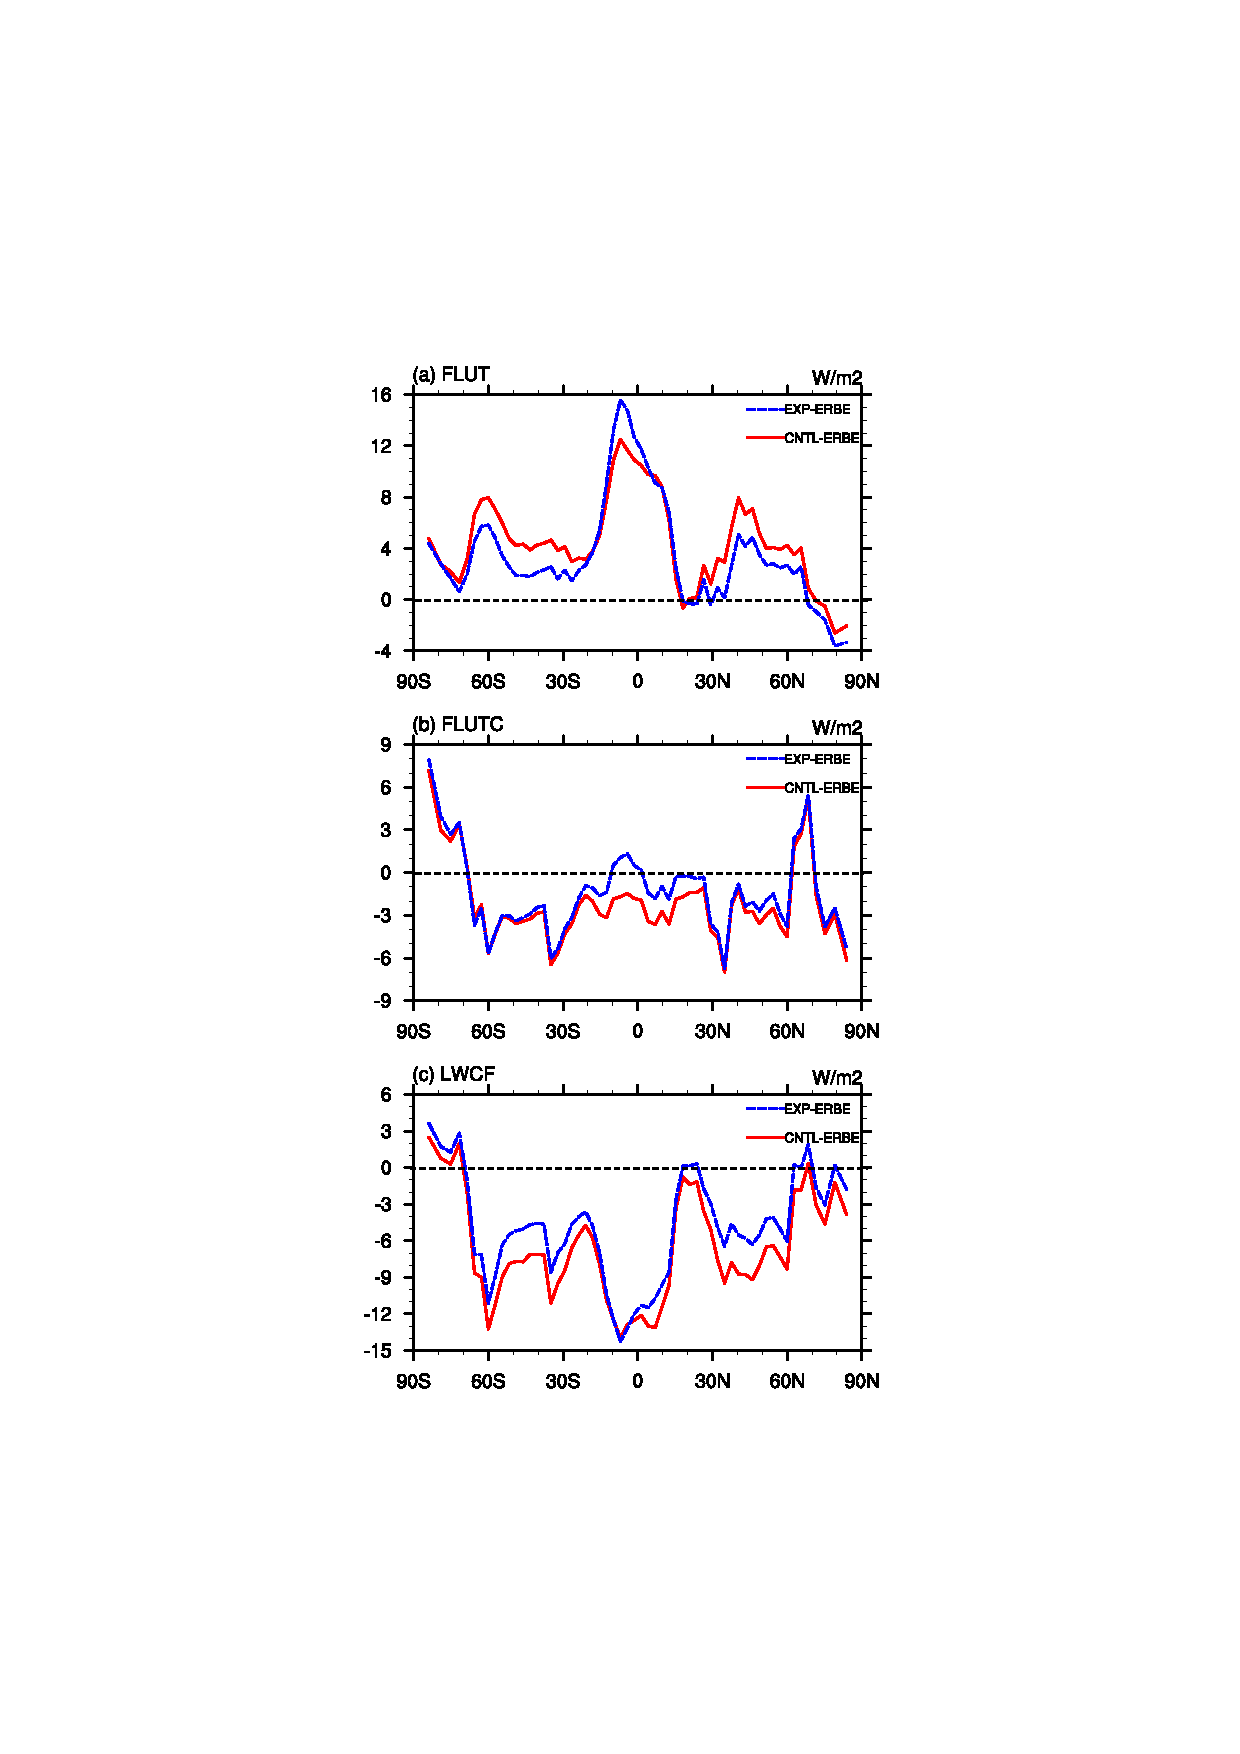
\includegraphics[width=12cm]{radiation_curve}
\caption{Meridional distributions of annual mean difference between EXP / CNTL and observation of FLUT (a), FLUTC (b), and LWCF (c).}
\end{figure}

\clearpage
%% TWO-COLUMN FIGURES

%f
%\begin{figure*}[t]
%\includegraphics[width=12cm]{FILE NAME}
%\caption{TEXT}
%\end{figure*}


%% TABLES
%%
%% The different columns must be seperated with a & command and should
%% end with \\ to identify the column brake.

%% ONE-COLUMN TABLE

%t

\begin{table}[t]
\caption{Initial selected uncertain parameters in GAMIL2}
\begin{tabular}{l l l c}
\tophline
Parameter & Description & Default & Range \\
\middlehline
c0 & rain water autoconversion coefficient for deep convection & 3.0e-4 & 1.e-4 $\sim$ 5.4e-3 \\
ke & evaporation efficiency for deep convection & 7.5e-6 & 5e-7 $\sim$ 5e-5 \\
capelmt & threshold value for cape for deep convection & 80 & 20 $\sim$ 200 \\
rhminl & threshold RH for low clouds & 0.915 & 0.8 $\sim$ 0.95 \\
rhminh & threshold RH for high clouds & 0.78 & 0.6 $\sim$ 0.9 \\
c0\_shc & rain water autoconversion coefficient for shallow convection & 5e-5 & 3e-5 $\sim$ 2e-4 \\
cmftau & characteristic adjustment time scale of shallow cape & 7200 & 900 $\sim$ 14400 \\
\bottomhline
\end{tabular}
\belowtable{} % Table Footnotes
\end{table}

\begin{table}[t]
\caption{Model output variables in the metrics}
\begin{tabular}{l l l l}
\tophline
Variable & Observation & Variable & Observation \\
\middlehline
Meridional wind at 850hPa   & ECMWF & Geopotential Z at 500hPa              & ECMWF \\
Meridional wind at 200hPa   & ECMWF & Total precipitation rate              & GPCP \\
Zonal wind at 850hPa        & ECMWF & Longwave cloud forcing                & ERBE \\
Zonal wind at 200hPa        & ECMWF & Shortwave cloud forcing               & ERBE \\
Temperature at 850hPa       & ECMWF & Long wave upward flux at TOA          & ERBE \\
Temperature at 200hPa       & ECMWF & Clearsky long wave upward flux at TOA & ERBE \\
Specific Humidity at 850hPa & ECMWF & Short wave net flux at TOA            & ERBE \\
Specific Humidity at 400hPa & ECMWF & Clearsky short wave net flux at TOA   & ERBE \\
\bottomhline
\end{tabular}
\belowtable{} % Table Footnotes
\end{table}

\begin{table}[t]
\caption{Fall factor samplings of parameters and metrics}
\begin{tabular}{l l l l l l l l l l l l}
\tophline
ID & c0 & rhminl & rhminh & cmftau & metrics & ID & c0 & rhminl & rhminh & cmftau & metrics \\
\middlehline
1  & 1.00E-04 & 0.915 & 0.78 & 7200 & 1.152 & 14 & 3.00E-04  & 0.875 & 0.78  & 7200  & 1.019     \\
2  & 3.00E-04 & 0.915 & 0.78 & 7200 & 1     & 15 & 3.00E-04  & 0.913 & 0.78  & 7200  & 1.007     \\
3  & 3.04E-04 & 0.915 & 0.78 & 7200 & 1.054 & 16 & 3.00E-04  & 0.95  & 0.78  & 7200  & 1.094     \\
4  & 5.08E-04 & 0.915 & 0.78 & 7200 & 1.017 & 17 & 3.00E-04  & 0.915 & 0.6   & 7200  & 1.00547   \\
5  & 7.13E-04 & 0.915 & 0.78 & 7200 & 0.987 & 18 & 3.00E-04  & 0.915 & 0.675 & 7200  & 1.027676  \\
6  & 9.17E-04 & 0.915 & 0.78 & 7200 & 1.01  & 19 & 3.00E-04  & 0.915 & 0.75  & 7200  & 1.023358  \\
7  & 1.12E-03 & 0.915 & 0.78 & 7200 & 1.04  & 20 & 3.00E-04  & 0.915 & 0.825 & 7200  & 1.028264  \\
8  & 1.33E-03 & 0.915 & 0.78 & 7200 & 1.044 & 21 & 3.00E-04  & 0.915 & 0.9   & 7200  & 1.160479  \\
9  & 2.55E-03 & 0.915 & 0.78 & 7200 & 1.075 & 22 & 3.00E-04  & 0.915 & 0.78  & 900   & 1.22922   \\
10 & 3.78E-03 & 0.915 & 0.78 & 7200 & 1.084 & 23 & 3.00E-04  & 0.915 & 0.78  & 4275  & 1.064064  \\
11 & 5.00E-03 & 0.915 & 0.78 & 7200 & 1.09  & 24 & 3.00E-04  & 0.915 & 0.78  & 7650  & 1.004806  \\
12 & 3.00E-04 & 0.8   & 0.78 & 7200 & 1.223 & 25 & 3.00E-04  & 0.915 & 0.78  & 11025 & 1.077167  \\
13 & 3.00E-04 & 0.838 & 0.78 & 7200 & 1.054 & 26 & 3.00E-04  & 0.915 & 0.78  & 14400 & 1.148265  \\
\bottomhline
\end{tabular}
\belowtable{} % Table Footnotes
\end{table}

\begin{table}[t]
\caption{Comparison with effective and efficiency}
\begin{tabular}{l l l l l}
\tophline
  & Optimal solution & $N_{step}$ & $N_{size}$ & Core hours \\
\middlehline
Down-hill simplex & 0.9585    & 80         & 1  & 14400 \\
PSO               & 0.911537  & 24         & 12 & 51840 \\
DE                & 0.942148  & 33         & 12 & 71280 \\
Dowmhill\_2\_steps  & 0.9256899 & 25+34    &  1 & 10620 \\
Downhill\_3\_steps  & 0.9098545 & 80+25+50 &  1 & 27900 \\
\bottomhline
\end{tabular}
\belowtable{} % Table Footnotes
\end{table}

\clearpage
%% TWO-COLUMN TABLE

%t
%\begin{table*}[t]
%\caption{TEXT}
%\begin{tabular}{column = lcr}
%\tophline

%\middlehline

%\bottomhline
%\end{tabular}
%\belowtable{} % Table Footnotes
%\end{table*}


%% NUMBERING OF FIGURES AND TABLES
%%
%% If figures and tables must be numbered 1a, 1b, etc. the following command
%% should be inserted before the begin{} command.

%\addtocounter{figure}{-1}\renewcommand{\thefigure}{\arabic{figure}a}


%% MATHEMATICAL EXPRESSIONS

%% All papers typeset by Copernicus Publications follow the math typesetting regulations
%% given by the IUPAC Green Book (IUPAC: Quantities, Units and Symbols in Physical Chemistry,
%% 2nd Edn., Blackwell Science, available at: http://old.iupac.org/publications/books/gbook/green_book_2ed.pdf, 1993).
%%
%% Physical quantities/variables are typeset in italic font (t for time, T for Temperature)
%% Indices which are not defined are typeset in italic font (x, y, z, a, b, c)
%% Items/objects which are defined are typeset in roman font (Car A, Car B)
%% Descriptions/specifications which are defined by itself are typeset in roman font (abs, rel, ref, tot, net, ice)
%% Abbreviations from 2 letters are typeset in roman font (RH, LAI)
%% Vectors are identified in bold italic font using \vec{x}
%% Matrices are identified in bold roman font
%% Multiplication signs are typeset using the LaTeX commands \times (for vector products, grids, and exponential notations) or \cdot
%% The character * should not be applied as mutliplication sign


%% EQUATIONS

%% Single-row equation

%\begin{equation}

%\end{equation}

%% Multiline equation



%\begin{align}
%& y=2+4x_1+4x_2-x_1^2-x_2^2+2sin(2x_1)sin(2x_2) \\
%& 0.5 \leq x_1, x_2 \leq 3.5
%\end{align}


%% MATRICES

%\begin{matrix}
%x & y & z\\
%x & y & z\\
%x & y & z\\
%\end{matrix}


%% ALGORITHM

\begin{algorithm}[htb]
\caption{Preprocessing the initial values of Downhill Simplex Algorithm} 
\label{alg:sequential-operation}
\begin{algorithmic}
%\STATE !********************************************
%\STATE !(1) Setting the initial values
%\STATE !******************************************** 
\STATE sampling\_sets=full\_factor\_sampling(parameters\_range)
\FOR{each initial $V_i$ of N+1 vertexes}
\STATE candidate\_init\_sets += min(i, sampling\_sets)
\ENDFOR
\WHILE{one parameter have the same values in the N+1 sets}
\STATE j=1
\STATE remove\_parameter\_set(the parameter set with higher metrics, candidate\_init\_sets)
\STATE candidate\_init\_sets += min(N+1+j, sampling\_sets)
\STATE j+=1
\ENDWHILE
\end{algorithmic}
\end{algorithm}

% \begin{algorithm}[htb]
% \caption{Downhill Simplex Algorithm} 
% \label{alg:sequential-operation}
% \begin{algorithmic}
% %\STATE !*********************************************
% %\STATE !(2) Downhill Simplex Algorithm
% %\STATE !*********************************************
% \WHILE {step=1,2..., until convergence}
% \STATE $V_h=$vertex with the highest metrics value
% \STATE $V_{l0}=$vertex with the lowest metrics value
% \STATE $V_{l1}=$vertex with the second lowest metrics value
% \STATE !***computing the center of gravity $V_g$ except for $V_h$***
% \STATE $V_g=\frac{1}{n}(\sum_{i=1}^{N+1} V_i - V_h)$ 
% \STATE !***computing the reflection vertex $V_r$ of $V_h$ based on $V_g$***
% \ENDWHILE
% \end{algorithmic}
% \end{algorithm}


%% CHEMICAL FORMULAS AND REACTIONS

%% For formulas embedded in the text, please use \chem{}

%% The reaction environment creates labels including the letter R, i.e. (R1), (R2), etc.

%\begin{reaction}
%% \rightarrow should be used for normal (one-way) chemical reactions
%% \rightleftharpoons should be used for equilibria
%% \leftrightarrow should be used for resonance structures
%\end{reaction}


%% PHYSICAL UNITS
%%
%% Please use \unit{} and apply the exponential notation

\end{document}
